\fontfamily{\sfdefault}\selectfont
% XCircuit output "discrete_pll_full_noise.tex" for LaTeX input from discrete_pll_full_noise.ps
\def\putbox#1#2#3#4{\makebox[0.00000in][l]{\makebox[#1][l]{}\raisebox{\baselineskip}[0.00000in][0.00000in]{\raisebox{#2}[0.00000in][0.00000in]{\scalebox{#3}{#4}}}}}
\def\rightbox#1{\makebox[0.00000in][r]{#1}}
\def\centbox#1{\makebox[0.00000in]{#1}}
\def\topbox#1{\raisebox{-0.60\baselineskip}[0.00000in][0.00000in]{#1}}
\def\midbox#1{\raisebox{-0.20\baselineskip}[0.00000in][0.00000in]{#1}}
   \scalebox{1}{
   \normalsize
   \parbox{6.30000in}{
   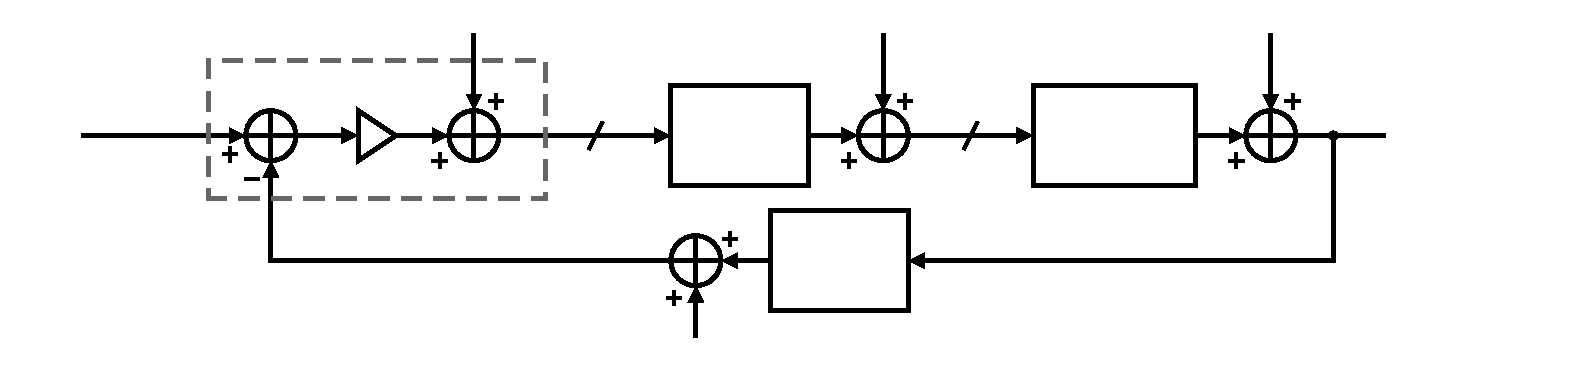
\includegraphics[scale=0.60000]{./figs/discrete_pll_full_noise.pdf}\\
   % translate x=416 y=544 scale 0.38
   \putbox{0.33600in}{1.00800in}{0.84}{$\Phi_{ref}$[n]}%
   \putbox{1.56000in}{0.51000in}{0.84}{$\Phi_{div}$[n]}%
   \putbox{2.27400in}{1.03200in}{0.84}{e$_\Phi$[n]}%
   \putbox{1.47000in}{1.07400in}{0.84}{\rotatebox{-360}{$\frac{\mathrm{M}}{2\pi}$}}%
   \putbox{1.20600in}{1.00800in}{0.84}{$\Phi_e$}%
   \putbox{0.83400in}{1.28400in}{0.84}{TDC}%
   \putbox{2.77200in}{0.89400in}{0.84}{H$_{LF}$(z)}%
   \putbox{3.79800in}{1.02000in}{0.84}{u[n]}%
   \putbox{4.22400in}{0.90600in}{0.84}{$\frac{2\pi K_{DCO}T}{1-z^{-1}}$}%
   \putbox{5.22000in}{0.99600in}{0.84}{$\Phi_{out}$[n]}%
   \putbox{3.22200in}{0.39600in}{0.84}{$\div$ N}%
   \putbox{4.13400in}{1.17000in}{0.84}{DCO}%
   \putbox{1.93200in}{1.30800in}{0.84}{q$_{n_{TDC}}$[n]}%
   \putbox{3.57000in}{1.30800in}{0.84}{q$_{n_{LF}}$[n]}%
   \putbox{2.82000in}{0.09600in}{0.84}{$\Phi_{n_{div}}$[n]}%
   \putbox{5.12400in}{1.30800in}{0.84}{$\Phi_{n_{DCO}}$[n]}%
   } % close 'parbox'
   } % close 'scalebox'
   \vspace{-\baselineskip} % this is not necessary, but looks better
\fontfamily{\rmdefault}\selectfont
